\section{Elementen als Torusknopen: Toewijzing van $T(p,q)$}

Onderstaande tabel koppelt de beschouwde elementen aan kandidaat-torusknopen $T(p,q)$. We vermelden per knoop het geschatte linking number $L_k$ (aantal zelf-omstrengelingen van de vortexlijnen) en bespreken isotopen waar relevant. Deze toewijzing is gebaseerd op minimale knoopcomplexiteit die de lading ($Z$) en massa van het element kan dragen binnen VAM~\cite{Kleckner2013KnotsVortex}.
% --- Figuur 1: 3D Torus Knoop ---
\begin{figure}[H]
    \centering
    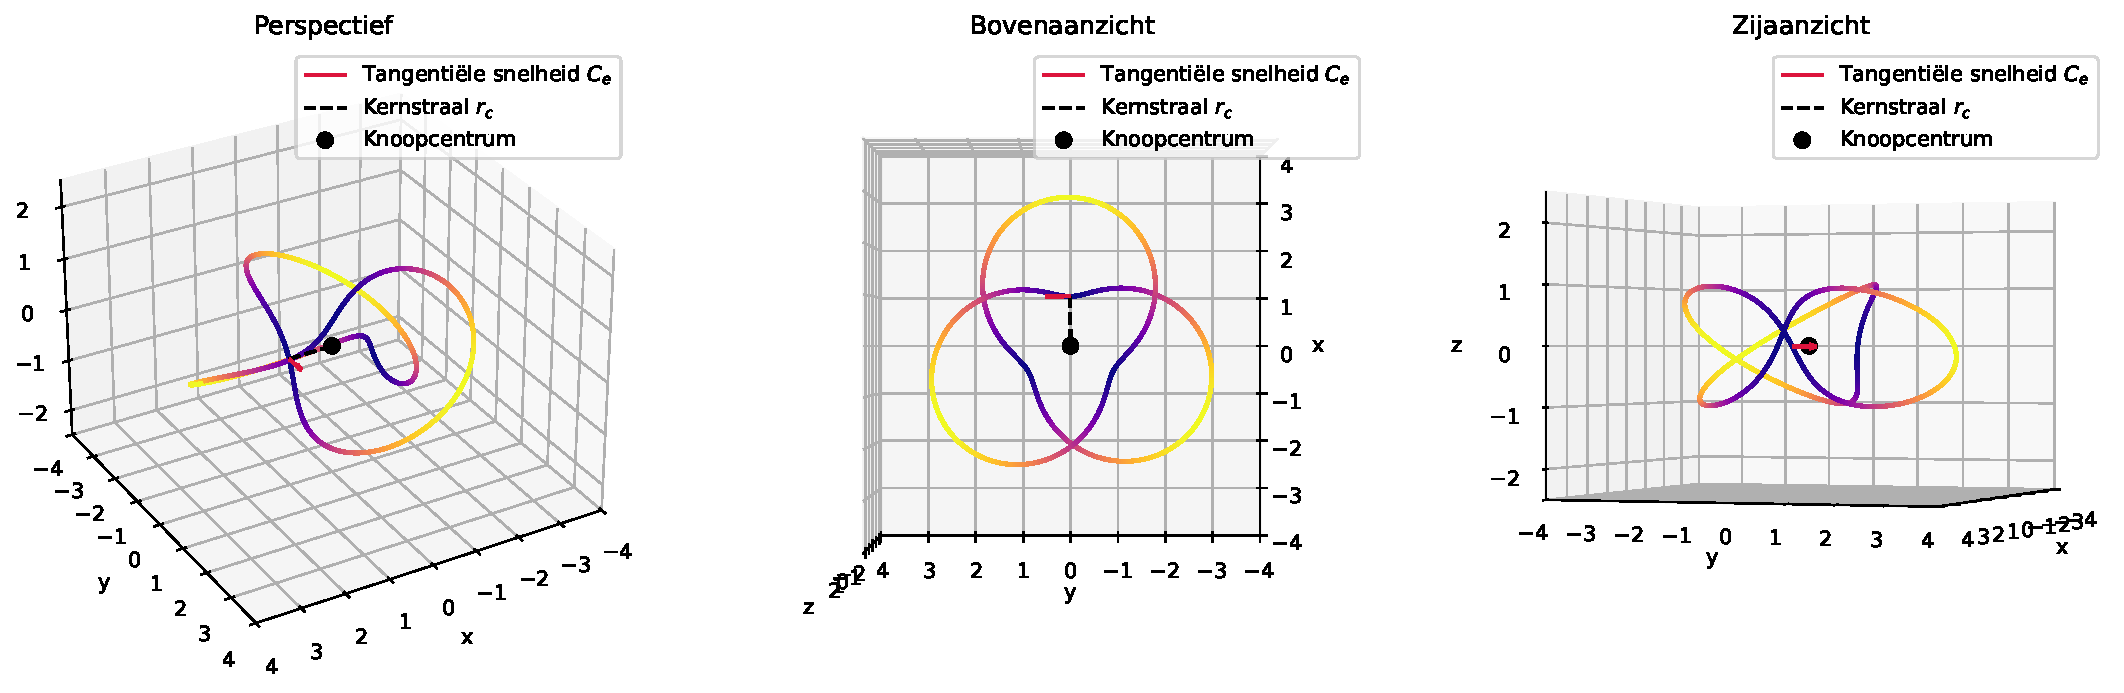
\includegraphics[width=0.65\textwidth]{../1_vortexknopen}
    \caption{De torusknoop $T(2,3)$ als basismodel voor waterstof in het Vortex Æther Model. De tangentiële snelheid $C_e$ en kernstraal $r_c$ worden visueel aangeduid.}
    \label{fig:torus_t23}
\end{figure}

\begin{table}[h!]
    \centering
    \begin{tabular}{lll}
        \hline
        Element (Z) & Voorgestelde torusknoop $T(p,q)$ & $L_k$ (helicititeit) en opmerkingen (isotopen)\\
        \hline
        Waterstof (1) & $T(2,3)$ (trefoilknoop)~\cite{Faddeev1997KnottedSolitions} & $3$, $^1$H basis; $^2$H extra neutron-binding nodig\\
        Helium (2) & $T(2,5)$ & $5$, $^4$He stabiel; $^3$He neutronvariatie\\
        Lithium (3) & $T(2,7)$ & $7$, $^7$Li meest stabiel; $^6$Li minder stabiel\\
        Beryllium (4) & $T(2,9)$ & $9$, $^9$Be stabiel; $^8$Be onstabiel (valt uiteen)\\
        Boor (5) & $T(2,11)$ & $11$, $^{11}$B stabiel; $^{10}$B stabiel met neutronvariatie\\
        Koolstof (6) & $T(2,13)$ & $13$, $^{12}$C zeer stabiel; $^{13}$C stabiele isotopenvariant\\
        IJzer (26) & $T(4,3)$ (voorbeeld) & $8$, $^{56}$Fe hoogste bindingsenergie, optimale knoopconfiguratie\\
        Uranium (92) & Complex (samengesteld) & –, $^{238}$U zwaar, borderline stabiel; composiet van subknopen\\
        \hline
    \end{tabular}
    \caption{Voorgestelde torusknopen voor enkele elementen binnen het Vortex Æther Model.}\label{tab:table}
\end{table}


% --- Figuur 2: Elementen vs Knoopstructuren ---
\begin{figure}[H]
    \centering
    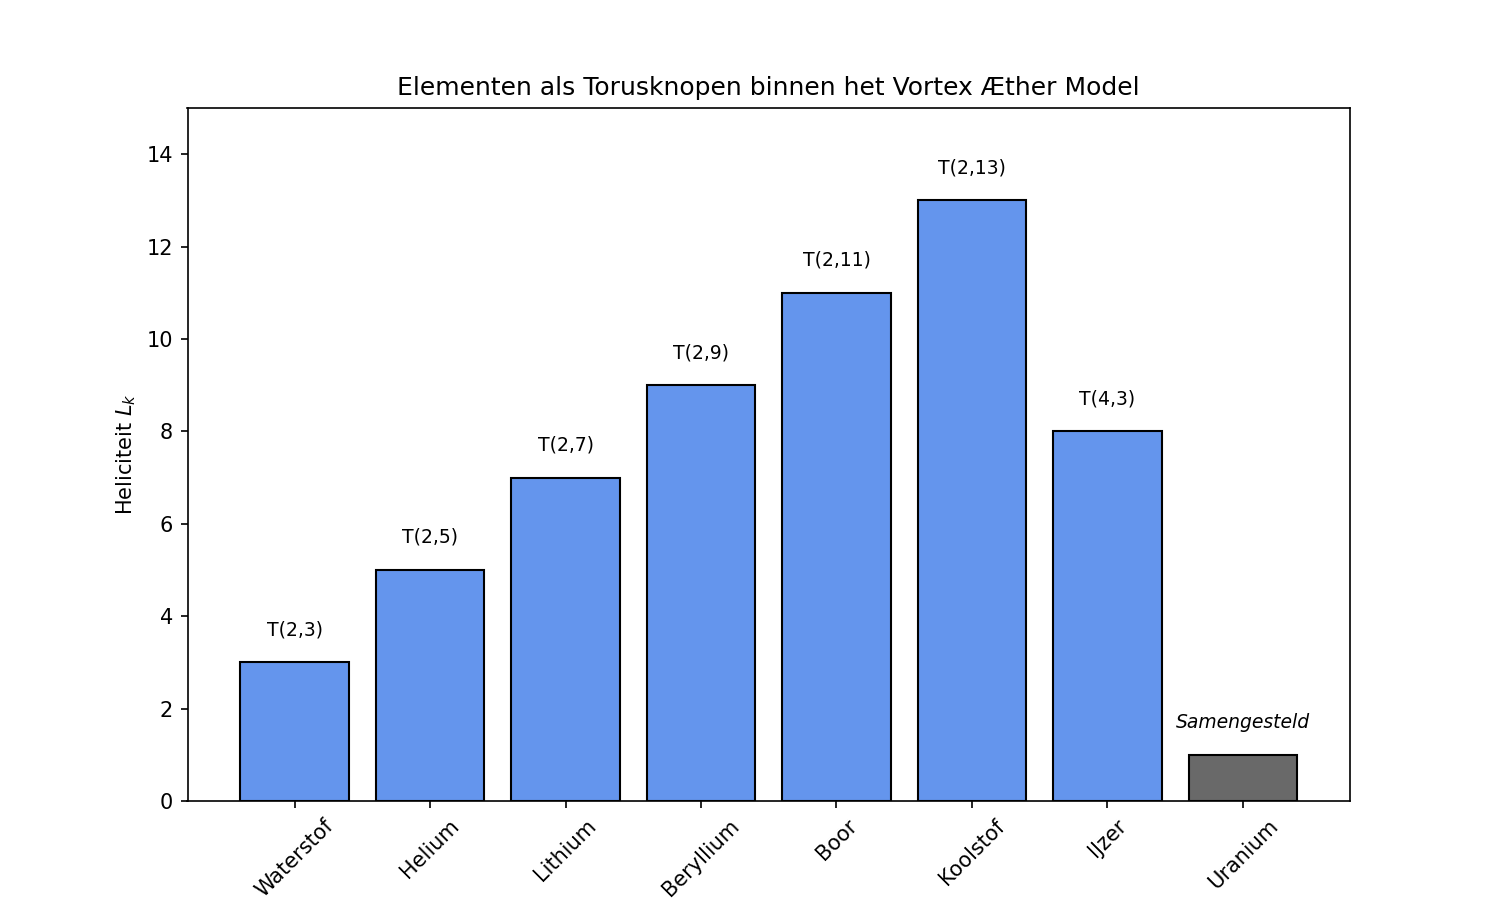
\includegraphics[width=0.7\textwidth]{../2_elementenTorusknopen}
    \caption{Aantal heliciteitskwanta $L_k$ per chemisch element. De torusknoopclassificatie geeft een topologisch alternatief voor het periodiek systeem.}
    \label{fig:elementen_torusknoop}
\end{figure}

\begin{figure}[H]
    \centering
    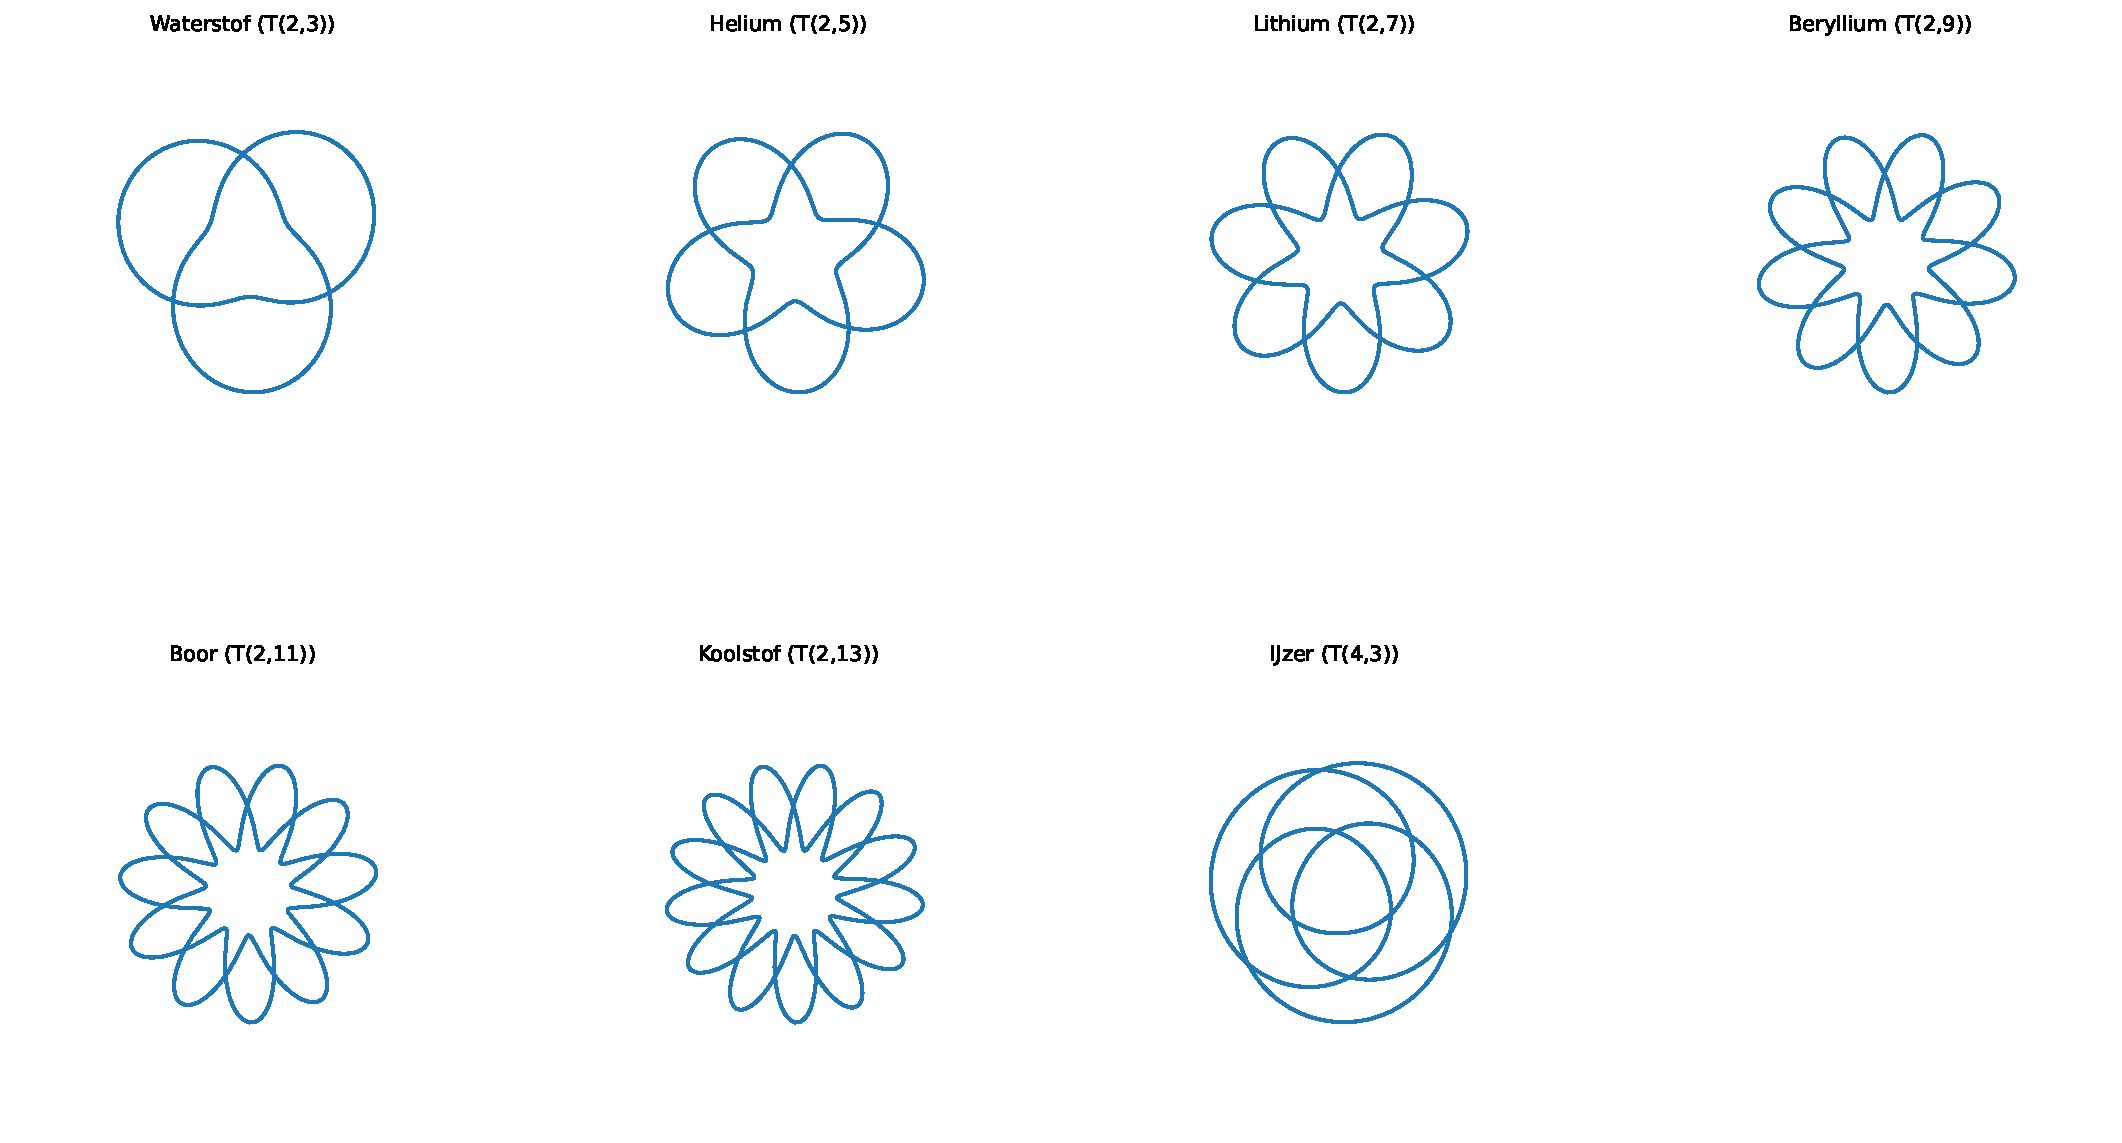
\includegraphics[width=0.8\textwidth]{../0_eersteKnopen}
    \caption[Torusknopen voor lichte elementen (bovenaanzicht)]{
        Bovenaanzicht van voorgestelde torusknopen \( T(p, q) \) binnen het Vortex Æther Model (VAM) voor de elementen:
        \textbf{Waterstof} \(T(2,3)\),
        \textbf{Helium} \(T(2,5)\),
        \textbf{Lithium} \(T(2,7)\),
        \textbf{Beryllium} \(T(2,9)\),
        \textbf{Boor} \(T(2,11)\),
        \textbf{Koolstof} \(T(2,13)\), en
        \textbf{IJzer} \(T(4,3)\).
        Elke knoop vertegenwoordigt een unieke heliciteit \( L_k \) die nodig is voor de interne wervelstabiliteit van het element binnen de Æther.
    }
    \label{fig:torusknopen_top}
\end{figure}


In waterstof (Z=1) stellen we de kern (proton) voor als de eenvoudigste niet-triviale vortexknoop: de trefoilknoop $T(2,3)$. De trefoil heeft topologisch $L_k=3$ omdat men het kan beschouwen als een gevlochten structuur van 2 strengen met 3 windingen. Binnen VAM correspondeert dit met de minimale heliciteit nodig om een ladingseenheid te dragen.

Isotopen zoals deuterium ($^2$H) zouden extra neutrale wervelstructuren bevatten, bijvoorbeeld als satellietknoop gekoppeld aan de protonknoop. Tritium ($^3$H) vereist analoog extra neutron-satellieten, wat overeenkomt met de instabiliteit in β-verval.

Helium (Z=2) wordt voorgesteld als $T(2,5)$ met $L_k \approx 5$. Voor helium geldt dat een hogere heliciteit noodzakelijk is voor voldoende centripetale druk tegen Coulomb-afstoting. Helium-4 heeft neutronen als interne extra wervelingen, terwijl helium-3 minder massa heeft door een afwijkende neutronconfiguratie.

Lithium (Z=3), voorgesteld als $T(2,7)$, volgt hetzelfde patroon. Lithium-7 is stabiel, lithium-6 iets minder door neutrontekort.

Beryllium (Z=4) als $T(2,9)$ is stabiel als $^9$Be, terwijl $^8$Be uiteenvalt in twee heliumkernen door onvoldoende massa-druk om de hoge heliciteit te stabiliseren.

Boor (Z=5) en koolstof (Z=6) vervolgen dit rijtje met respectievelijk $T(2,11)$ en $T(2,13)$, met diverse stabiele isotopen binnen dezelfde knoopfamilie. Koolstof-12 onderscheidt zich door bijzondere stabiliteit, mogelijk door symmetrische knoopconfiguratie.

\usepackage{tabularx} % In je preambule voor automatische kolombreedte

\begin{table}[H]
    \centering
    \caption[Elementen als torusknopen in het VAM]{Toewijzing van torusknopen \( T(p,q) \) aan lichte elementen binnen het Vortex Æther Model. De heliciteit \( L_k \) representeert het aantal interne vortex-omstrengelingen.}
    \label{tab:torusknopen}
    \begin{tabularx}
        \hline
        \( Z \) & Element & \( T(p,q) \) & Heliciteit \( L_k \) en opmerkingen \\
        \hline
        1 & Waterstof & \( T(2,3) \) & \( L_k = 3 \), trefoilknoop, basale protonstructuur \\
        2 & Helium & \( T(2,5) \) & \( L_k = 5 \), extra neutronbinding in \( ^4\text{He} \) \\
        3 & Lithium & \( T(2,7) \) & \( L_k = 7 \), \( ^7\text{Li} \) stabiel, neutrontekort in \( ^6\text{Li} \) \\
        4 & Beryllium & \( T(2,9) \) & \( L_k = 9 \), \( ^9\text{Be} \) stabiel, \( ^8\text{Be} \) valt uiteen \\
        5 & Boor & \( T(2,11) \) & \( L_k = 11 \), neutronvariant in \( ^{10}\text{B} \) \\
        6 & Koolstof & \( T(2,13) \) & \( L_k = 13 \), \( ^{12}\text{C} \) zeer stabiel door symmetrie \\
        26 & IJzer & \( T(4,3) \) & \( L_k = 8 \), hoogste bindingsenergie bij \( ^{56}\text{Fe} \) \\
        \hline
    \end{tabularx}
\end{table}

Zoals weergegeven in figuur~\ref{fig:torusknopen_top} en tabel~\ref{tab:torusknopen}, kent elk licht element binnen het VAM een specifieke torusknoopstructuur toe die de topologische basis vormt voor zijn massa, stabiliteit en isotopie.


IJzer (Z=26) markeert een overgang naar complexere knopen zoals $T(4,3)$, die een optimale configuratie biedt voor de hoogste bindingsenergie.

Uranium (Z=92) is complex en samengesteld, niet meer voorstelbaar als één torusknoop maar eerder als composiet van subknopen, consistent met het waargenomen fissiegedrag van zware elementen.

\begin{figure}[H]
    \centering
    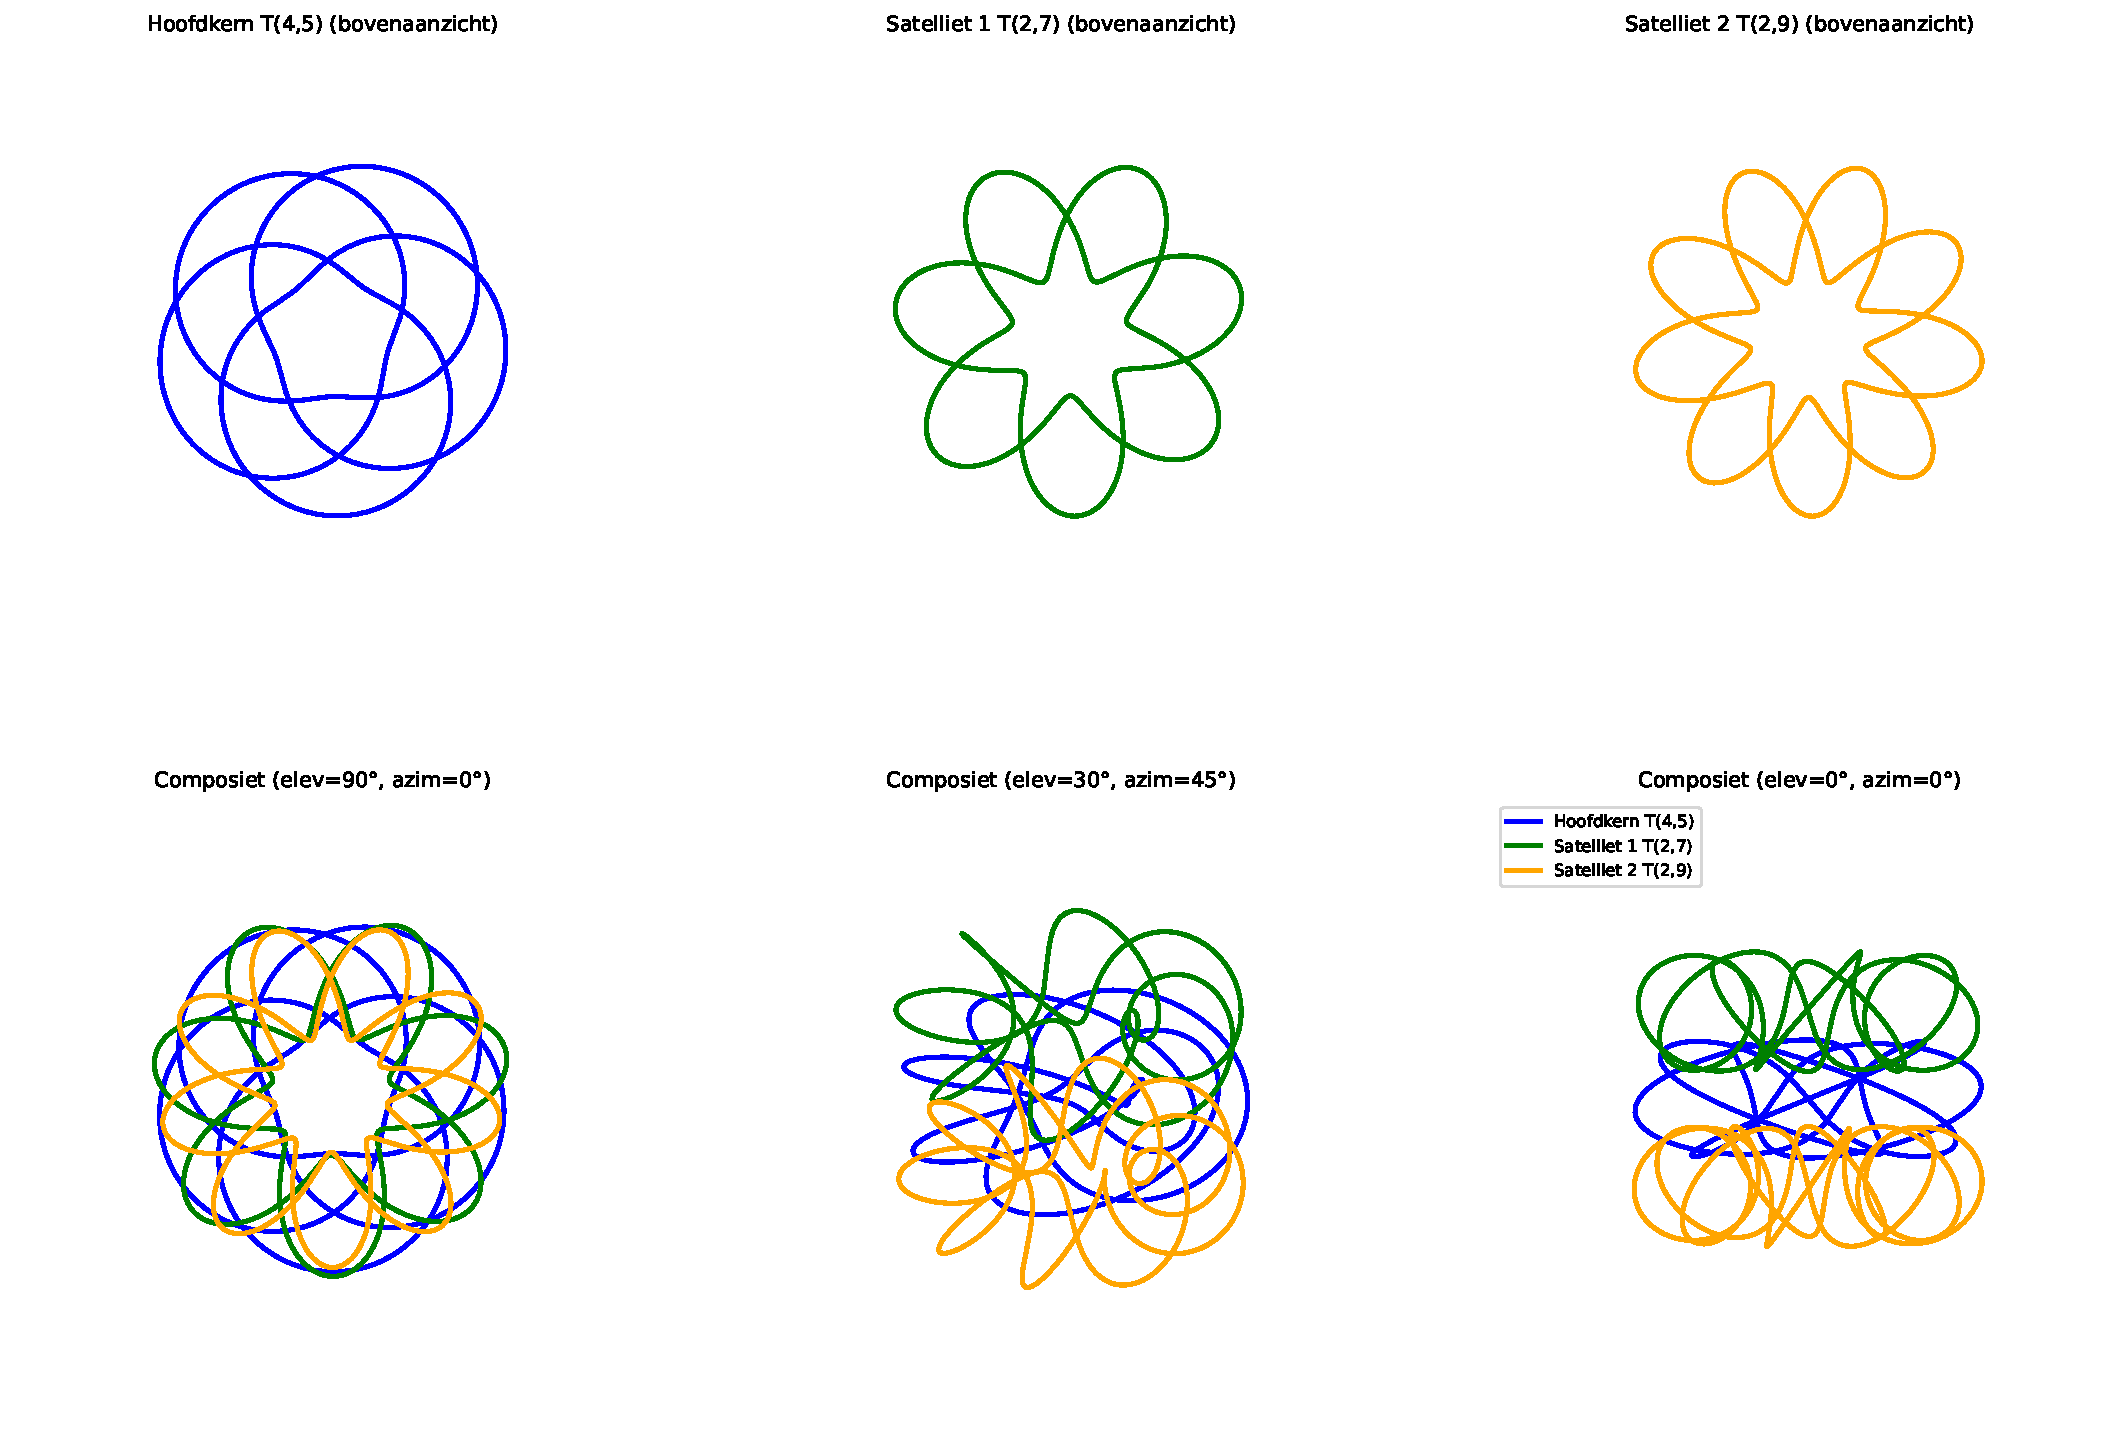
\includegraphics[width=\textwidth]{images/0_UraniumKnoop}
    \caption[Samengestelde vortexstructuur van uranium-238 in VAM]{
        Visualisatie van de voorgestelde samengestelde vortexstructuur van uranium-238 binnen het Vortex Æther Model (VAM).
        \textbf{Bovenste rij}: individuele torusknopen in bovenaanzicht:
        de \textcolor{blue}{hoofdkern \(T(4,5)\)}, de \textcolor{green}{satellietknoop \(T(2,7)\)} en de \textcolor{orange}{satellietknoop \(T(2,9)\)}.
        \textbf{Onderste rij}: drie perspectieven op de volledige composietstructuur met duidelijke interactie tussen de knopen.
        Deze topologische decompositie verklaart de hoge heliciteit, bindingsenergie, en splijtbaarheid van zware kernen.
    }
    \label{fig:uranium_2x3}
\end{figure}

\begin{table}[H]
    \centering
    \caption[Samengestelde vortexstructuur van uranium-238]{Voorstel voor een samengestelde vortexconfiguratie voor uranium-238 in VAM, opgebouwd uit geneste torusknopen. De totale heliciteit wordt dan:
        $ L_k^\text{totaal} = L_k^{(4,5)} + L_k^{(2,7)} + L_k^{(2,9)} = 20 + 7 + 9 = 36 $\\
        Met aanvullende interactietermen zoals linking, nesting, of mutual writhing:
        $ L_k^\text{eff} = L_k^\text{totaal} + \Delta L_\text{interactie} $
    waar $\Delta L_\text{interactie} \approx 3\text{–}5$ afhankelijk van configuratie. Dit reproduceert de hoge bindingsenergie en instabiliteit (fissiegevoeligheid) van zware elementen.
    }
    \label{tab:uranium_knoopstructuur}
    \begin{tabularx}{\textwidth}
        \hline
        Substructuur & \( T(p,q) \) & \( L_k \) & Functie binnen kernstructuur \\
        \hline
        Hoofdkern & \( T(4,5) \) & 20 & Draagt hoofdheliciteit en basale bindingsenergie \\
        Satelliet 1 & \( T(2,7) \) & 7 & Neutroncluster ter massa-aanvulling \\
        Satelliet 2 & \( T(2,9) \) & 9 & Drukbalans en stabilisatie \\
        Interactiecomponent & – & \( \Delta L \approx 3{-}5 \) & Inter-knoop interacties (linking, nesting) \\
        \hline
        \textbf{Totaal} & – & \( \approx 39{-}41 \) & Geschatte effectieve heliciteit \\
        \hline \\
    \end{tabularx}
\end{table}